% alt + shift + 1
% make projname.pdf
% wordcount: detex writeup.tex | wc -w

\documentclass[12pt]{article}
%------------------------Dimensions----------------------------

\topmargin=0.0in
\oddsidemargin=0.0in           % 1in margins at left and right
\evensidemargin=0in
\textwidth=6.5in               % US paper is 8.5in wide
\marginparwidth=0.5in

\headheight=0pt                % 1in margins at top and bottom
\headsep=0pt
\topmargin=0in
\textheight=9.0in              % US paper is 11.0in high

%adjustments...
\addtolength{\topmargin}{-0.5in}
\addtolength{\textheight}{1.0in}
\addtolength{\textwidth}{0.5in}
\addtolength{\oddsidemargin}{-0.25in}
\addtolength{\evensidemargin}{-0.25in}
                       
\pagestyle{empty}

%------------------------Packages----------------------------
\usepackage{textcomp}
\usepackage{longtable}
\usepackage{setspace}
\usepackage{amsmath,amssymb,amsthm}
\usepackage{graphicx}
\usepackage{epsfig}
\usepackage{subfig}
\usepackage[paperwidth=8.5in,paperheight=11in,margin=0.98in]{geometry}
\usepackage{listings,float}
\usepackage{color}
\usepackage{array}
\usepackage{cancel}
\usepackage[numbers]{natbib}

%------------------------Commands----------------------------
\newcommand{\be}{\begin{enumerate}}
\newcommand{\ee}{\end{enumerate}}
\newcommand{\bi}{\begin{itemize}}
\newcommand{\ei}{\end{itemize}}
\newcommand{\bv} {{\bf v}}
\newcommand{\bD} {{\bf D}}

\definecolor{listinggray}{gray}{0.9}
\definecolor{lbcolor}{rgb}{0.9,0.9,0.9}
\lstset{
	tabsize=4,
	rulecolor=,
	language=matlab,
	keywords={break,case,catch,continue,else,elseif,end,for,function,
      global,if,otherwise,persistent,return,switch,try,while},
        basicstyle=\footnotesize\ttfamily,
        upquote=true,
        aboveskip={1.5\baselineskip},
        columns=fixed,
        showstringspaces=false,
        extendedchars=true,
        breaklines=true,
        prebreak = \raisebox{0ex}[0ex][0ex]{\ensuremath{\hookleftarrow}},
        frame=single,
        showtabs=false,
        showspaces=false,
        showstringspaces=false,
        identifierstyle=\ttfamily,
        keywordstyle=\color[rgb]{0,0,1},
        commentstyle=\color[rgb]{0.133,0.545,0.133},
        stringstyle=\color[rgb]{0.627,0.126,0.941},
}

\captionsetup{width=.75\textwidth} 

\begin{document}
\pagestyle{plain} %pagenumbers
\title{CSCI 4/5576: The Random Logistic Map}
\date{December 16, 2014}
\author{Amy Le (5576)\\Long Tat (4576)\\Emily Bertelson (4576)\\Kristina Entzel (4576)}
\maketitle
\section{Abstract}
The purpose of this investigation was to explore and simulate a
spatially random logistic map using a dynamic load balancer on Janus, the CU
supercomputer \cite{janus}. The recursive nature of the map prevents the individual
fixed point iterations from being parallelized, but a set of
iterations may be load balanced over many cores. The original simulation was written in serial code in
MATLAB. Our solution has modified the original version for efficiency,
speed, and scalability. We implemented our simulation in C++ and present our
results in terms of a histogram of observed periodic orbits and a
bifurcation diagram. Single core optimization techniques,
such as SIMD loop vectorization and function inlining, as well as
using a dynamic load balancer for more efficient work distribution
were applied. The HDF5 file format was used to store the simulation results in a better archival format. The benchmarking (weak scaling study) results imply the best
speedup and efficiency is gained when invoking the load balancer on
one node (12 cores), although we tested our simulation over 16 nodes
(192 cores). Improvements to this project include optimizing the
post-simulation data processing. 
\newpage
\section{Introduction}
\subsection{Deterministic case}
\hspace{5mm}The Logistic map is a quadratic recursive equation on the domain
[0,1]. It is a popularly studied topic in nonlinear dynamics and has
applications in population modeling. There is one parameter in the
expression, $r$, which can take any value in the range [0,4]. 
\begin{equation*}
x_{n+1} = rx_n(1-x_n)
\end{equation*}
\begin{figure}[H]
	\begin{center}
		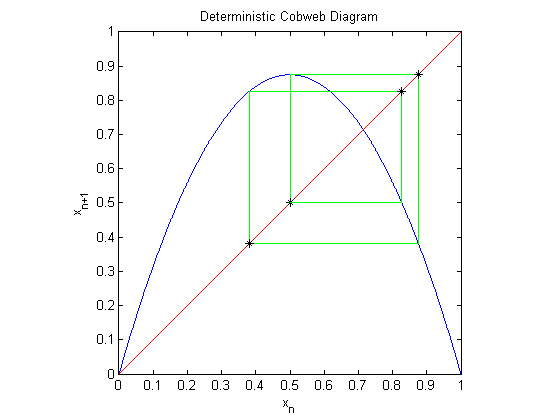
\includegraphics[scale=0.7]{det_cobweb}
\caption{Deterministic Logistic Map (blue) for $r=3.2$. There is a stable period
4 orbit. The order of the period is calculated by counting the number
of crossings (green) on the line $x_{n+1}=x_n$ (red). Between $r \in [0,3.5]$, we observe stable periodic orbits.}
	\end{center}
\end{figure}
\begin{figure}[H]
	\begin{center}
		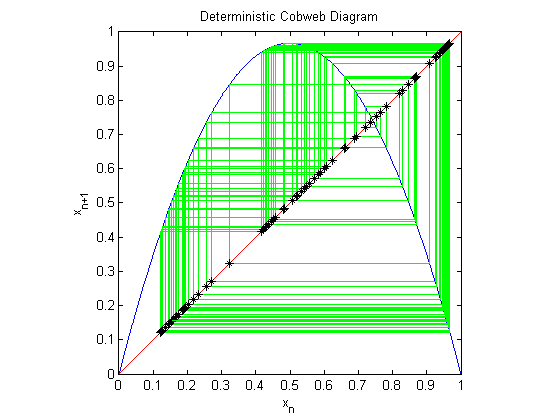
\includegraphics[scale=0.7]{chaos}
\caption{Deterministic Logistic Map (blue) for $r=3.8$. There is a no
  stable orbit. For values of $r \in [3.5,4]$, the system experiences the onset of
chaos.}
	\end{center}
\end{figure}
There are two ways to vary the deterministic map. We can simulate the
parameter $r$ as a function of time or space. The existing literature
explore the notion of randomness in time, so we explore $r$ as a
function of space \cite{athreya}.
\subsection{Random case}
The following equation is the fixed point iteration that the code
completes, where $R(x)$ is calculated by manipulating a random number generator.
\begin{equation*}
x_{n+1} = R(x_n)x_n(1-x_n)
\end{equation*}
The exact details of how to calculate $R(x)$ are outlined below.
\begin{align}\label{randlog}
\begin{split}
\ln(R(x)) &= \xi(x)\\
\xi(x) &= \ln(r) + 2\sum^N_{n=1}a_n\cos(2\pi nx)-b_n\sin(2\pi nx)\\
a_n,b_n &\sim Unif(-M_n,M_n)\\
M_n &= \sqrt{1.5S_n}\\
S_n &= \alpha e^{-L|n|}\\
\alpha &= \sigma^2 \tanh(L/2)\\
\sigma &< \ln(4/r)\frac{\tanh(L/4)}{\sqrt{1.5\tanh(L/2)}}
\end{split}
\end{align}
Where $L \in (0,1)$ represents the correlation length (and is fixed
for each simulation) and $r \in [0,4]$ is also fixed for each
simulation. 
\begin{figure}[H]
	\begin{center}
		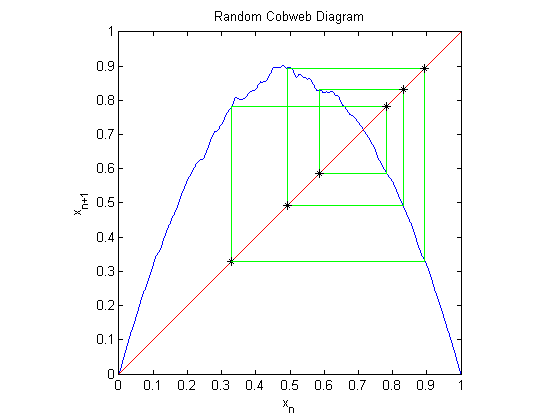
\includegraphics[scale=0.7]{rand_cobweb}
\caption{One instance of a random logistic map (blue). The map has
  converged to a stable period 6 orbit (green). Notice the
  ``wiggliness'' in the parabola shape.}
	\end{center}
\end{figure}
Other instances of the random map would vary from this realization,
due to the random nature of the map. 
\begin{figure}[H]
	\begin{center}
		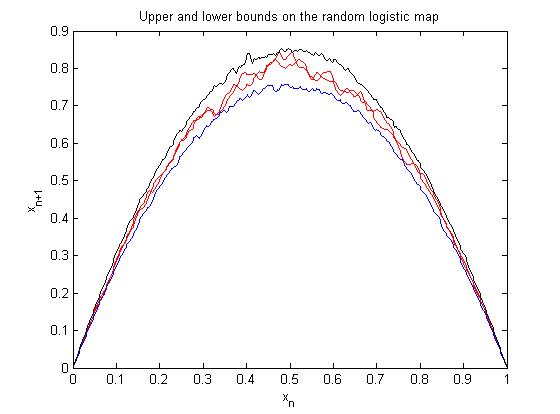
\includegraphics[scale=0.7]{envelope}
\caption{A coarse demonstration of the upper (black) and lower (blue) bounds of the
  random logistic map. Sample realizations are shown in red.}
	\end{center}
\end{figure}
\subsection{Project Goals}
Since the map can take on a range of values for any given position in
space, it would be useful to characterize some of its properties. In particular, we will be studying the stability of the map,
which includes locating fixed points and generating bifurcation
diagrams. The two main goals are:
\be
\item Find the expected number of order $p$ periodic orbits for a
  the random map ($p = 1, 2, 3, ...$)
\be
\item For an initial starting value $x_0 \in [0,1]$ and a specific
  random function $R_0(x)$, iterate until you
  find the fixed point(s), $x_i^*$ associated with $R_0(x)$. 
\item Classify the fixed points in terms of a period $p$ orbit. 
\item Each processor should take a different initial $x_0$ and report
  whether the initial condition led to finding a unique stable orbit  
\bi
\item The processors should be properly load balanced.
\item As each processor finishes its work, it will write its results
  to an HDF5 file (parallel i/o)
\ei
\item Repeat the above steps for a large number of different random
  maps $R_i(x)$, $i = 0, 1, 2,... \bar{N}$ in order to find the expected
  number of order $p$ periodic orbits for the random map.
\ee
\item Create a set valued bifurcation diagram \cite{lamb}
\be
\item For many values of $r \in [0,4]
$, and a fixed random function
  $R_0(x)$, plot the locations of the periodic orbits as a function of
  $r$. A period $p$ orbit will have $p$ corresponding $x$ values as
  its orbit locations (e.g. a period 1 orbit will have 1 fixed point,
  a period 2 orbit will have 2 fixed points, and so on). 
\bi
\item Use a HDF5 file to store the simulation data and as a source to generate
  bifurcation diagrams
\ei
\ee
\ee
As the map has an element of randomness to it, many
simulations (a large $\bar{N}$) would be required for statistical analysis. 
\section{Method}
\hspace{5mm} After profiling the MATLAB code, we realized that our critical path is
the fixed point iteration calculation, so parallelizing our solver is
the necessary step to improve our performance. Unlike the problems we
encountered in class, we did not have a matrix or an array which we
can decompose and distribute to multiple processors. Our solver uses
the previous calculation to compute the current calculation. This
dependency renders parallelization with OpenMP/MPI impossible. 

Upon carefully reviewing our objective, we noticed that this project
was originally designed to collect data over a range of inputs. If
parallelizing at the file level is impossible, we parallelize
the project at the simulation level. This is possible because the
fixed point iterations are independent over a range of initial
conditions. A load balancer suits our purposes perfectly because the
load balancer will redistribute work over many processors to eliminate
wait time. The general progression of the project is outlined below:
\be
\item Convert the MATLAB code to C++
\item Confirm the C++ versions of the code that we each produce work
  together correctly by comparing to the serial version
\item Invoke the load balancer to assign an initial condition to each
  fixed point iteration 
\item Benchmark: strong scaling study (speedup and efficiency)
\ee

\begin{figure}[H]
	\begin{center}
		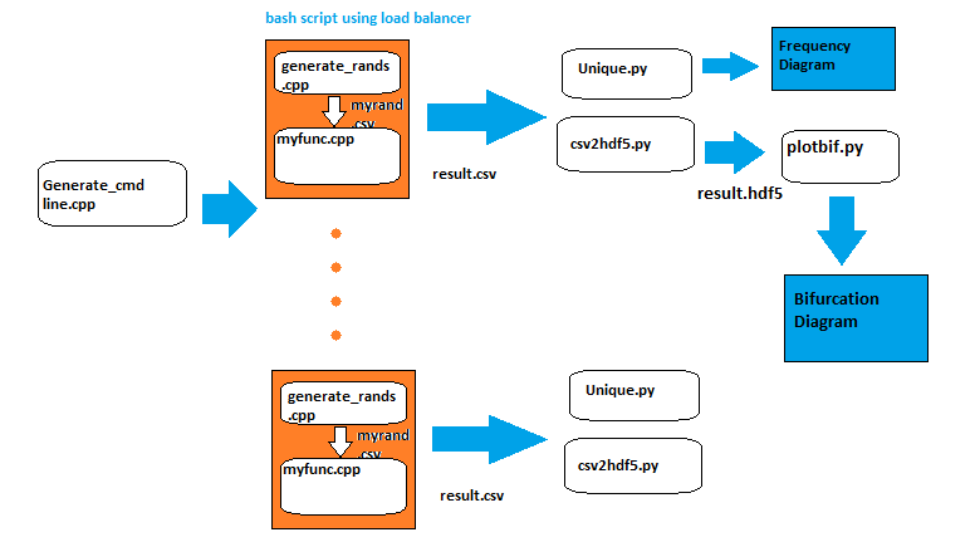
\includegraphics[scale=0.5]{workflow}
\caption{Workflow}\label{workflow}
	\end{center}
\end{figure}

The Workflow (Figure \ref{workflow}) demonstrates that the program
begins with \texttt{generate\_cmdlines.exe}. We start with
\texttt{generate\_cmdlines.exe} file which is the set up file for our
simulation.
\be
\item \texttt{generate\_cmdlines.exe}: This file will take 4 inputs (L,dr,dx,iter). It will generate all the bash script files. 
\item Bash Script files: Each of these scripts will invoke
\texttt{generate\_rands.exe} once which will take in with the same L
given in \texttt{generate\_cmdlines.exe}, an $r$ value which is
uniformly distributed between 0 and 4 with step size $dr$ and an output
file. This outfile contains the randomized parameters $a,b$, used by
\texttt{myfunc.exe}. This script also invokes the load balancer which
will distribute tasks over the available processors\footnote{Each task
  corresponds to executing \texttt{myfunc.exe} with a unique set of
  parameters: $L,r,x_0,a,b$. Different initial conditions $x_0$ are
  uniformly distributed between 0 and 1 with step size $dx$}.
\item \texttt{generate\_rands.exe}: Generate randomized parameters $a,b$ and put it into an output file for given $L$ and $r$ values.
\item \texttt{myfunc.exe}: Run the fixed point iteration and print out
  the orbit locations if they exist or return nothing if the map
  diverges. All output from \texttt{myfunc.exe} will be fed into a \texttt{result.csv} associated with that bash script file. Note that we can concatenate all these result files if we want to study the map's behavior as a whole. 
\item \texttt{csv2hdf5.py}: Convert \texttt{result.csv} to a HDF5 file
  while using \texttt{unique.py} to check for uniqueness in the data
  set. Save the processed data in an HDF5 file for archival
  purposes. \texttt{unique.py} also creates a histogram of the data.
\item \texttt{plotbif.py}: Use the HDF5 file to produce the bifurcation diagram. 
\ee

\subsection{Original Serial Implementation in MATLAB}
\hspace{5mm} Since MATLAB is inherently slower than C++, we expect seeing the code
speedup simply from porting the code to C++. Besides being written in serial, the code was slow due to some
inefficient I/O practices. After running a fixed point iteration, the
code would create a file and write the results to it. In other words,
for every fixed point iteration, that corresponds with an initial
condition $x_0$ and a parameter value $r$, a new file is
created. Furthermore, the data written was not checked until after all
files were created for uniqueness and convergence. Diverging cases
where no period orbit was found would create a file full of junk
data. The data processing steps included reopening all the data files,
removing duplicates, and sorting. 

To solve these practices we processed the data before writing to a
single csv file to avoid writing diverging orbits to the file. To
check uniqueness, we opened the csv file once, and checked line by line
(each line is a set of data) for uniqueness while comparing to an
array (in memory) that kept track of the unique data points. If the
data was unique, it was added to the array. These practices resulted
in a smaller set of data that was more manageable to graph.

\subsection{Single Core Optimization}
Optimizations implemented in the code conversion:
\bi
\item The aforementioned inefficient I/O practices were optimized
\item Preferential use of the multiply and add operators where possible, since
they are less expensive than divide and subtract operators
\item Used a reduction on the loop that computes the Fourier Series
  in order to take advantage of the data parallelism with SIMD
\item Loop structure was reorganized to take advantage of C++ being
  row-oriented (outer loop should go by rows, then inner loops go by columns)
\item Inlining in the C++ code to reduce the number of function calls
\item The lack of a built in uniform random number generator that generates a random
double between two doubles led to the creation of a psudeo random number
generator with the use of \texttt{rand} and \texttt{srand}.
\lstinputlisting{rand_ex.m}
\ei
\subsection{Load Balancer}
\begin{figure}[H]
	\begin{center}
		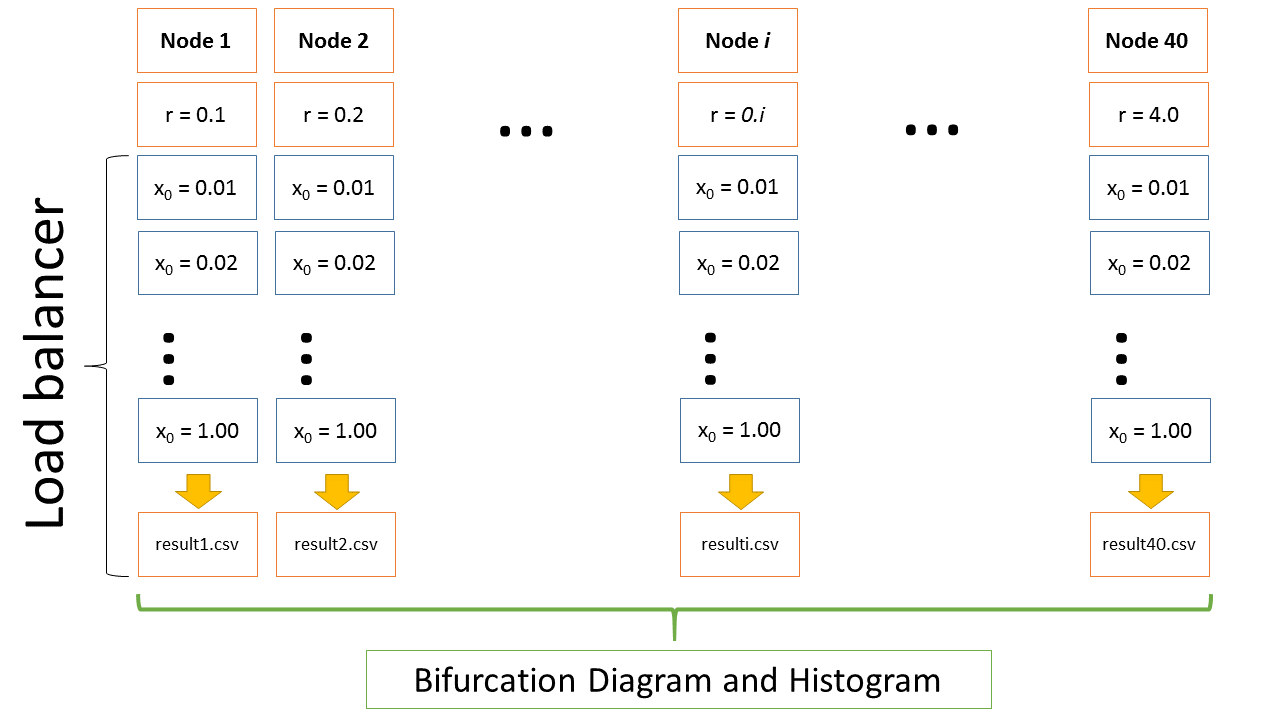
\includegraphics[scale=0.4]{load_balancer}
\caption{A load balancer recognizes the number of processors that are going to be used and manages the workload distribution among them. It first assigns all processors a chunk of work, and when a processor finishes the load balancer assigns that processor more work.}
	\end{center}
\end{figure}
\hspace{5mm} We researched types of load balancers \cite{olivier}. We found there
are many strategies for load balancing, such as sender initiated
diffusion, receiver initiated diffusion, hierarchical balance model, etc. \cite{dlb}. This investigation
used the Load Balance tool on Janus, which invokes a master-slave
strategy for balancing \cite{janus}. 

During fixed point iteration, we take a starting value, perform initial calculations, and then use this guess solution to find the next guess, and so on. Each iteration's solution is dependent on the previous iteration's solution, so this calculating the fixed period orbit for a starting point must be done in serial. 
Some starting values will converge to a fixed period orbit much more
quickly than others, and some starting values will diverge, and never
find a fixed period orbit  at all. The fixed point iteration for a
starting value is completely independent from another starting value,
so we can parallelize this by assigning each processor a starting
value to process. This allows us to optimize despite having a variety
of runtimes. 

First we assign a global $r$ to a node, then a starting value $x_0$ to
each processor. The diverging calculations will take place on
processors in parallel to converging calculations on other processors
and no time is wasted waiting. When a processor has either found a
solution or run through the 1000 iterations\footnote{The ceiling
  number of iterations we applied to any given initial condition is
  1000 iterates.} it stops the calculation and writes the resulting
fixed period orbits to a csv for that node. 

\subsubsection{Write Locks}
\hspace{5mm}Originally we had a single csv file for the entire program
where results would be written to. We ran simulations with different
initial $r$ and $L$ values across many nodes and wrote all the fixed
period orbits into a single csv file along with the accompanying
simulation parameters, $r$ and $L$. This practiced caused unexpected
I/O problems. The load balancer manages the workload of all processors
specified in slurm's \texttt{\#SBATCH -N} parameter. However, when we
used many different instances of the load balancer (invoking the load
balancer on different sets of jobs, each one independent of the
other), we observed erratic results due to multiple processors from
different jobs trying to write to the same file. This means the load
balancer tool invoked on independent jobs did not communicate between
the jobs, so upon finding a fixed period orbit, would write to the csv
file with no consideration of synchronization. The resulting csv was
an unreadable jumble of partial lines of solutions from different
nodes\footnote{Upon further reflection, this seems like a logical
  consequence of calling the load balancer over independent
  runs.}. One possible solution is to implement a system of write
locks, so that only one processor from any given run may write to the
file at a time. However, this has the potential to create a bottleneck
for our program. Therefore, we pursued a different strategy.

We resolved this issue by assigning a unique result file to each
instance that we called the load balancer on. Even though we ended up
creating as many files as we had nodes, this is still a massive
improvement in the I/O and number of files created from the original
implementation. Our final algorithm created $N$ files over $N$ nodes,
whereas the original implementation created $1000*N$ files over $N$ values
of $r$ and 1000 initial conditions.
\subsection{HDF5}
\hspace{5mm} While the output was initially stored in a
comma-separated value format, the HDF5 file format was chosen for
final storage of the data. An intermediary step (\texttt{unique.py})
removes redundancies from the .csv file before copying the data into
an HDF5 file (via \texttt{csv2hdf5.py}). Two resources were used to
implement the HDF5 aspect of the project \cite{folk} \cite{UserGuide}. 

The hierarchical structures allowed by the HDF5 format were ideal for our uses. We developed a structure with the intention of making the data convenient and efficient to access for the production of a bifurcation diagram and histogram, as well as future analysis.

The folowing is the structure of the output HDF5 file. Two groups
within the root store the data twice, in different formats; group
\texttt{arch} is used for plotting histograms, while group
\texttt{bif} stores three-dimensional coordinates for plotting
bifurcation diagrams.

\begin{tabbing}
\texttt{arch}\\
	\hspace{5mm} group ``$r$'' \\
		\hspace{10mm} group ``$L$'' \\
		\hspace{15mm} group ``$p=1$'' \\
				\hspace{20mm} dataset \\
					\hspace{25mm} $ (x_{1})$ \\
					\hspace{25mm} $ (x_{2})$ \\
					\hspace{25mm} $ (x_{3})$ \\
					\hspace{25mm} ... \\	
			\hspace{15mm} group ``$p=2$'' \\
				\hspace{20mm} dataset \\
					\hspace{25mm}                           $(x_{11},x_{12})$ \\
					\hspace{25mm} $(x_{21},x_{22})$ \\
					\hspace{25mm} ... \\
\end{tabbing}

\begin{tabbing}
\texttt{bif}\\
  \hspace{5mm} group ``$L$'' \\
  \hspace{10mm} dataset \\
  \hspace{15mm} $ (x_{1}, r, p=1)$ \\
  \hspace{15mm} $ (x_{1},x_2, r, p=2)$ \\
  \hspace{15mm} ... \\
  \hspace{15mm} $ (x_{1},x_2,...x_k, r, p=k)$ \\
\end{tabbing}

\section{Results}
\hspace{5mm} The results of the two sets of data give us the following
histograms and bifurcation diagrams. If our implementation is correct,
the results using the load balancer and C++ will strongly resemble the
results from the original MATLAB code. The nature of the equation
makes the exact replication of a single run difficult; the problem
involves random noise. Before implementing the ability to apply
extreme constraints to the parameters, we could not replicate a single
run, but preliminary results appeared as expected and were accepted as
correct.  

Further work after the presentation hardcoding the random coefficients into the C++ and Matlab code resulted in identical output and tested the correctness of our converted code.

Results from running the program in  Matlab are slightly different for each simulation but seem follow a general pattern, which is the subject of the study. 
\begin {table}[H]
\begin{center}
\begin{tabular}{ p{8cm} p{8cm}}    
\begin{center}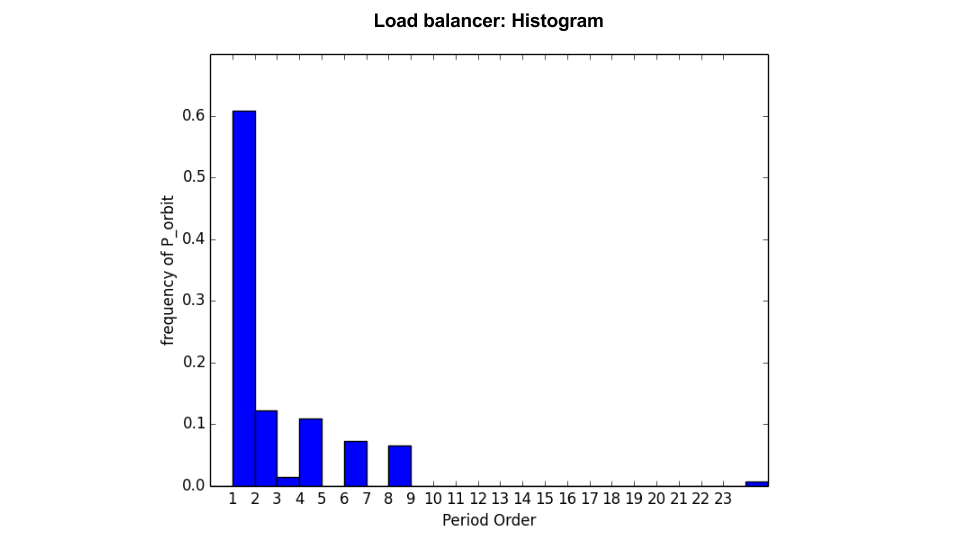
\includegraphics[scale=0.3]{hist}\end{center}&\begin{center} 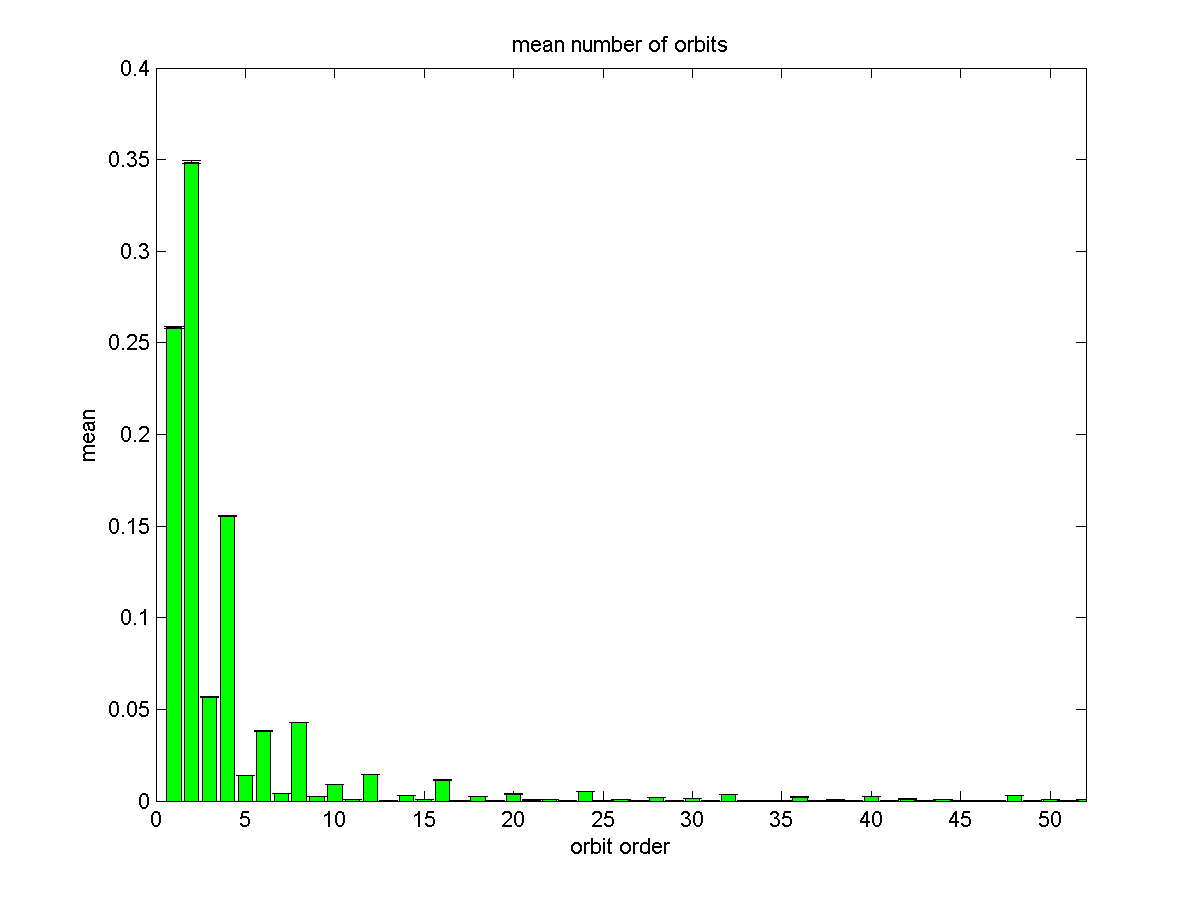
\includegraphics[scale=0.4]{serial_hist}\end{center}
\end{tabular}
\caption {Load balanced histogram (left) and Serial histogram
  (right). The histograms display the frequency of different period order orbits for given $r$ and $L$ values. They both indicate a tendency toward a high frequency of low order period orbits with few high order outliers.} \label{hist}
\end{center}
\end {table}

\begin {table}[H]
\begin{center}
\begin{tabular}{ p{8cm} p{8cm}}    
\begin{center}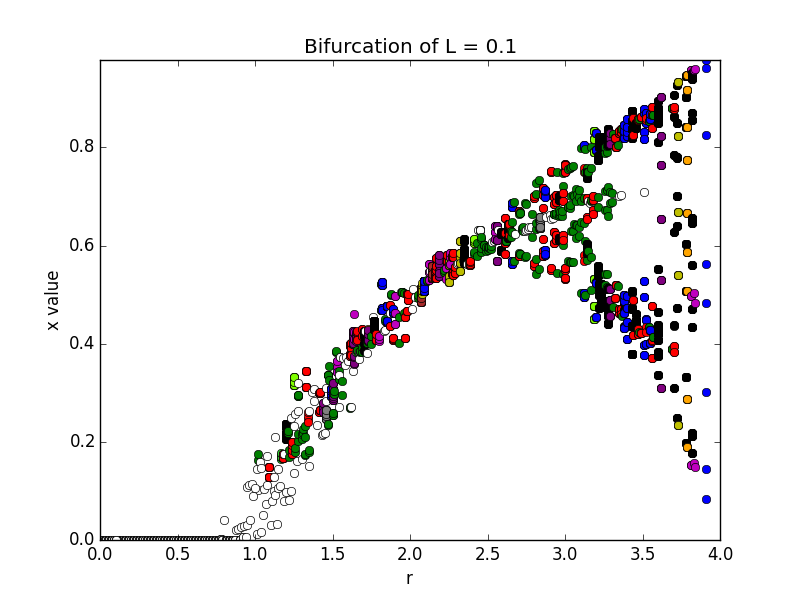
\includegraphics[scale=0.4]{Bifurcation_L1}\end{center}&\begin{center} 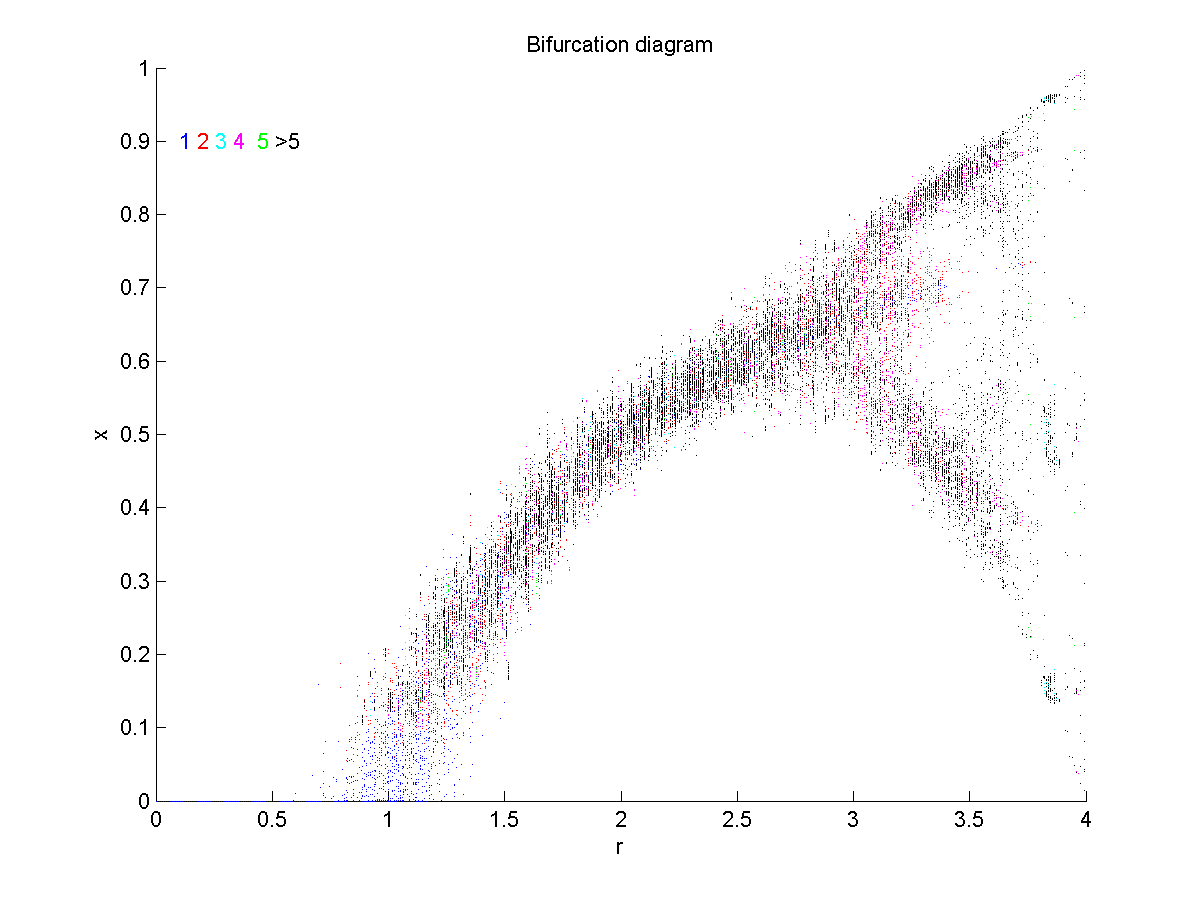
\includegraphics[scale=0.4]{bif}\end{center}
\end{tabular}
\caption {Load balanced Bifurcation with $L=0.1$ (left) and Serial
  Bifurcation with $L=0.1$ (right). The bifurcation diagrams plot the
  variable $r$ versus the resulting $x$ values for a given $L$. We
  observe bifurcations from the load balanced implementation occurring
  in similar places as the serial implementation.
} \label{bif}
\end{center}
\end {table}

 \begin{figure}[H]
	\begin{center}
		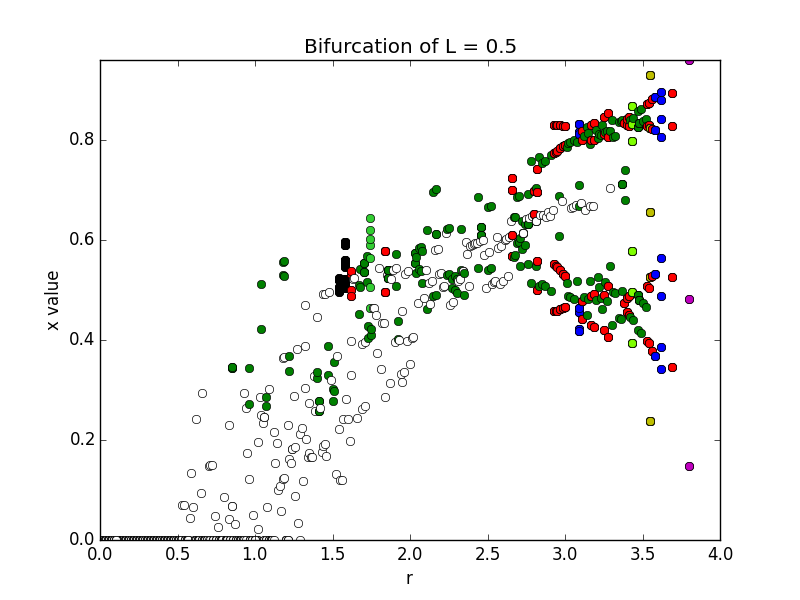
\includegraphics[scale=0.5]{Bifurcation_L5}
\caption{Bifurcation with $L=0.5$. Increasing the correlation length
  $L$ from 0.1 to 0.5 results in a very different bifurcation
  diagram. The correlation length affects the distribution of the
  random parameters by causing them to decrease exponentially
  (equation $S_n$ in (\ref{randlog})).}\label{lb_bif_5}
	\end{center}
\end{figure}

\subsection{Benchmarking}
\hspace{5mm} The original code written in MATLAB took hours to run a
simulation, and the optimized version of the code with the load
balancer ran in approximately 30 minutes. The benchmarking was
computed using the C++ code for homogeneity. We tested the code over
16 nodes (192 processors). 

Running the simulation to generate a bifurcation diagram requires choosing a number of $r$ values you want to graph and running the fixed point
  iteration on a set of values for that $r$ and an associated set of
  random coefficients. This means executing
  \texttt{generate\_rands.exe} for each $r$ to get the correct
  coefficients. The fixed problem size for benchmarking was testing 40
  $r$ values between [0,4], and 1000 initial conditions $x_0$ in [0,1]
  for each value of $r$.

For the serial run,
  \texttt{generate\_rands.exe} was called 40 times and each initial
  condition executed serially. For the parallel cases we increase the number of nodes used (from 1 node to 16 nodes), run
\texttt{generate\_rands.exe} over each value of $r$ and call the load
balancer which will distribute the work among the increased number of
processors.

We found that the best Speedup and Efficiency occurred for one node
(12 processors), though we may expect better Speedup and performance
with more $r$ values tested (perhaps on the order of 100 instead of 40). It is possible the communication overhead was high in proportion to the amount of work given to each processor due to only finding the solution or 40 values of $r$.
\begin{figure}[H]
	\begin{center}
		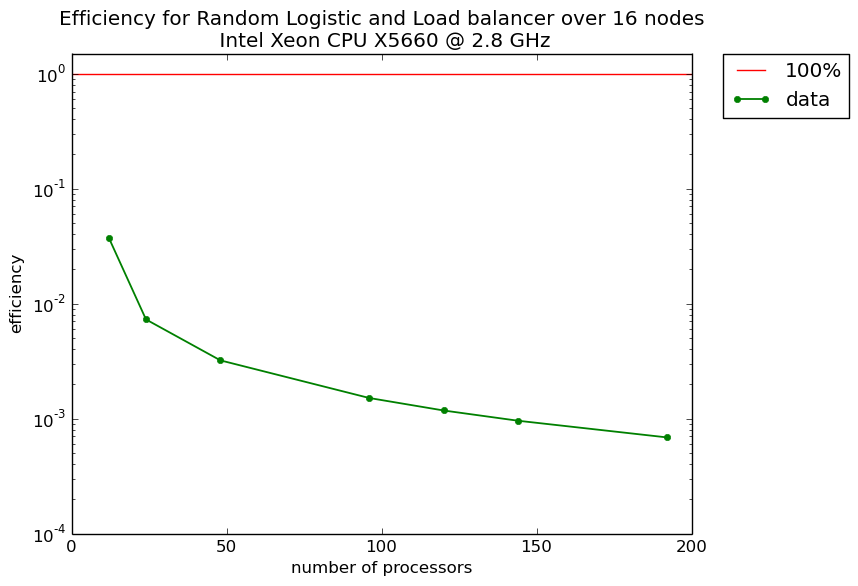
\includegraphics[scale=0.5]{efficiency_random_logistic}
\caption{Efficiency of our code. We found that the best Efficiency occurred for one node
(12 processors).}
	\end{center}
\end{figure}
\begin{figure}[H]
	\begin{center}
		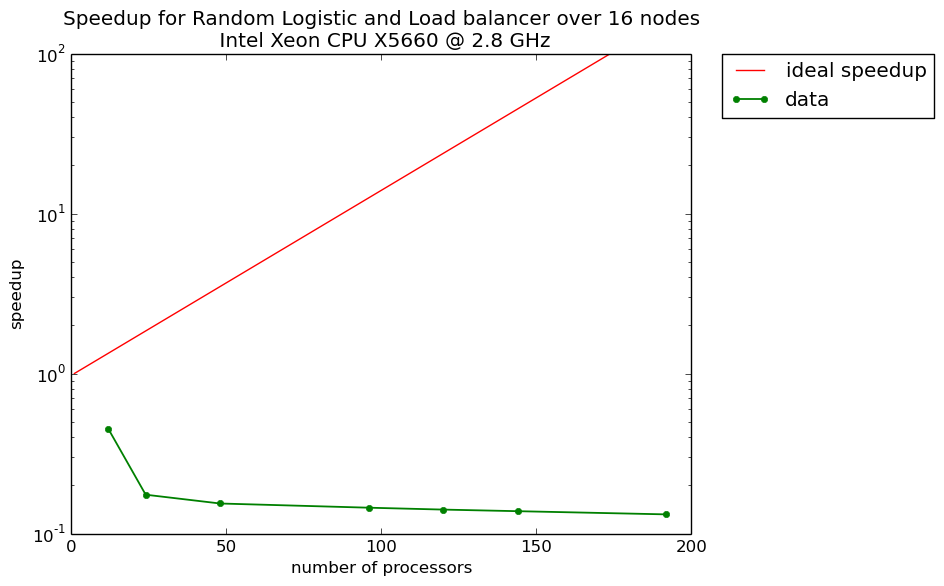
\includegraphics[scale=0.5]{speedup_random_logistic}
\caption{Speedup of our code. We found that the best Speedup occurred for one node
(12 processors).}\label{speedup}
	\end{center}
\end{figure}

\section{Conclusion}
Overall, the results of this investigation were positive. Since the
serial and load balanced versions of the simulation fall in relatively
the same range of values (Table \ref{hist}, and Table \ref{bif}), we believe the load-balanced versions output the
accurate results. The histograms give us an idea of the sort of
periodic orbits that occur most frequently in the random logistic
map. Table \ref{hist} shows that the
most commonly observed orbit is period 1. The bifurcation diagrams
demonstrate the periodic orbits are highly affected by the correlation
length $L$ in the simulation. It seems that for larger values of $L$,
eg. $L=0.5$ (Figure \ref{lb_bif_5}), there are fewer high order
periodic orbits than for lower values of $L$, eg. $L=0.1$ (Table \ref{bif}). This is indicated by the
larger density of white circles on the plot (white circles represent
period 1).
\subsection{Future Work}
\subsubsection{Post-simulation processing}
Our group focused more on the single-core optimization and dynamic
load balancing aspects of the simulation than on how to most
efficiently process the simulation data for generating the bifurcation
diagram and histogram. Some improvements we could work on in the
future would be to explore how to best remove duplicate orbits (as
more than one initial condition can converge to the same periodic
orbit) as we write the data to the HDF5 file. Another improvement
would be to use the link properties of the HDF5 file format to link
the data for each bifurcation diagram together, making a new ``view''
of the data for each kind of bifurcation diagram. 
\subsubsection{Scaling Study}
It was surprising that the speedup (Figure \ref{speedup}) plot showed
the optimal number of nodes is one. We suspect this may be due to the
fixed problem size we assigned to each set of nodes. Perhaps if the
problem size (number of initial conditions $x_0$ = number of tasks for
the load balancer) were larger, we would see a speedup graph that
increases over some nodes and then plateaus for too many nodes. This
investigation used 1,000 tasks, but a future scaling study would
increase the number of tasks to about 10,000 or more.
\newpage
\bibliographystyle{apa}
\bibliography{annot}

\end{document}
